\documentclass[aspectratio=169,10pt]{beamer}

\usetheme{Madrid}
\usecolortheme{default}
\setbeamertemplate{navigation symbols}{}
\setbeamertemplate{footline}[frame number]

\usepackage{amsmath,amssymb,booktabs}
\usepackage{graphicx}
\usepackage{hyperref}
\usepackage{fontspec}
\setmainfont{Noto Sans CJK SC}
\setsansfont{Noto Sans CJK SC}
\setmonofont{Noto Sans CJK SC}
\usepackage{tikz}
\usetikzlibrary{arrows.meta,positioning,decorations.pathreplacing,shapes.geometric,fit,backgrounds,calc,matrix,shapes.multipart}

% Semantic colors
\definecolor{positive}{HTML}{0173B2}
\definecolor{negative}{HTML}{DE8F05}
\definecolor{emphasis}{HTML}{029E73}
\definecolor{neutral}{HTML}{808080}
\definecolor{tableHeader}{HTML}{0173B2}
\definecolor{tableRow}{HTML}{F0F7FB}
\newcommand{\pos}[1]{\textcolor{positive}{#1}}
\newcommand{\con}[1]{\textcolor{negative}{#1}}
\newcommand{\HL}[1]{\textcolor{emphasis}{#1}}
\newcommand{\pkk}[1]{\textbf{#1}}
\newcommand{\fld}[1]{\textcolor{neutral}{#1}}

\title{乐器租赁管理系统}
\subtitle{数据库应用设计 — PPT 示例}
\author{AI Architect}
\date{2026-06-07}

\begin{document}

% ============================================================
% SLIDE 1: Title
% ============================================================
\begin{frame}
  \titlepage
  \vspace{-8pt}
  \begin{center}
    {\small Spring Boot 3 + PostgreSQL 15 + Vue 3 + 微信小程序}
  \end{center}
\end{frame}

% ============================================================
% SLIDE 2: Architecture Overview
% ============================================================
\begin{frame}{系统架构总览}
  \vspace{4pt}
  \begin{columns}[T]
    \column{0.35\textwidth}
    \begin{block}{前端层 (Presentation)}
      \begin{itemize}
        \item \textbf{Vue 3} 管理后台
        \item \textbf{微信原生小程序} 用户端
        \item Element Plus UI 组件库
      \end{itemize}
    \end{block}
    \vspace{4pt}
    \begin{block}{中间件}
      \begin{itemize}
        \item \textbf{Redis 7} — 分布式锁、缓存
        \item \textbf{RabbitMQ} — 异步通知队列
        \item \textbf{Quartz} — 定时任务调度
      \end{itemize}
    \end{block}

    \column{0.60\textwidth}
    \begin{block}{服务层 (Spring Boot 3.x 单体)}
      \begin{itemize}
        \item \textbf{Controller} — REST API 接口
        \item \textbf{Service} — 业务逻辑（库存、预约、支付、通知）
        \item \textbf{Repository} — Spring Data JPA 数据访问
        \item \pos{JWT Auth + 全局异常处理}
      \end{itemize}
    \end{block}
    \vspace{4pt}
    \begin{block}{数据层}
      \textbf{PostgreSQL 15} — 13 张业务表 + Flyway 版本迁移
    \end{block}
  \end{columns}
\end{frame}

% ============================================================
% SLIDE 3: Database ER Diagram (Core)
% ============================================================
\begin{frame}{核心数据模型 (ER 关系)}
  \vspace{-2pt}
  \begin{center}
    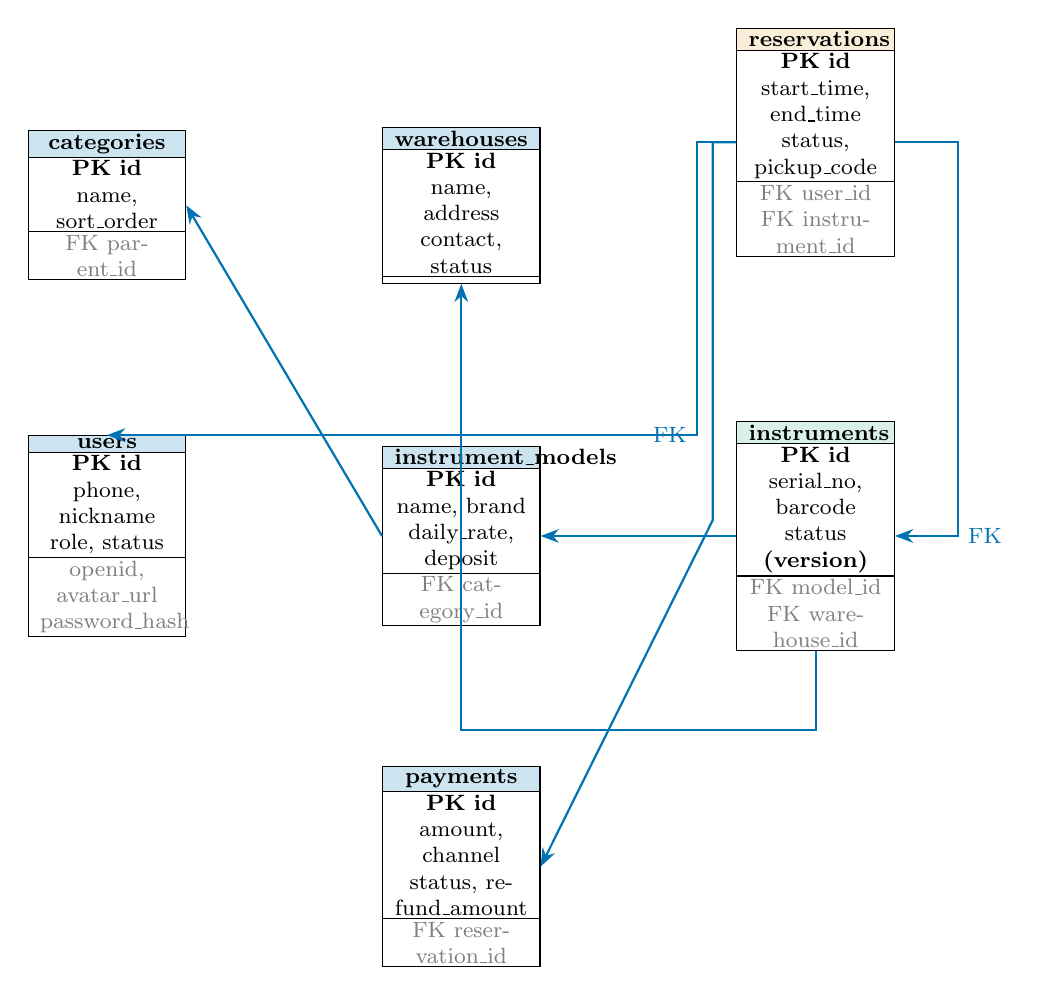
\begin{tikzpicture}[
      entity/.style={rectangle split, rectangle split parts=3, draw,
                     rectangle split part fill={tableHeader!20,white,white},
                     minimum width=2.0cm, font=\footnotesize,
                     text width=1.7cm, align=center, inner sep=1pt},
      pk/.style={font=\footnotesize\bfseries},
      fld/.style={font=\footnotesize, text=neutral},
      edge/.style={-{Stealth}, thick, positive},
      re/.style={<->, thick, negative, dashed}
    ]
      % Users
      \node[entity, rectangle split part fill={positive!20,white,white}] (u) at (0, 0) {
        \textbf{users}
        \nodepart{second}
        \textbf{PK id} \\
        phone, nickname \\
        role, status
        \nodepart{third}
        \fld{openid, avatar\_url} \\
        \fld{password\_hash}
      };

      % Warehouse
      \node[entity] (wh) at (4.5, 4.2) {
        \textbf{warehouses}
        \nodepart{second}
        \textbf{PK id} \\
        name, address \\
        contact, status
        \nodepart{third}
        \fld{}
      };

      % instrument_models
      \node[entity] (im) at (4.5, 0) {
        \textbf{instrument\_models}
        \nodepart{second}
        \textbf{PK id} \\
        name, brand \\
        daily\_rate, deposit
        \nodepart{third}
        \fld{FK category\_id}
      };

      % instruments
      \node[entity, rectangle split part fill={emphasis!15,white,white}] (ins) at (9, 0) {
        \textbf{instruments}
        \nodepart{second}
        \textbf{PK id} \\
        serial\_no, barcode \\
        status \textbf{(version)}
        \nodepart{third}
        \fld{FK model\_id} \\
        \fld{FK warehouse\_id}
      };

      % reservations
      \node[entity, rectangle split part fill={negative!15,white,white}] (r) at (9, 5) {
        \textbf{reservations}
        \nodepart{second}
        \textbf{PK id} \\
        start\_time, end\_time \\
        status, pickup\_code
        \nodepart{third}
        \fld{FK user\_id} \\
        \fld{FK instrument\_id}
      };

      % payments
      \node[entity] (p) at (4.5, -4.2) {
        \textbf{payments}
        \nodepart{second}
        \textbf{PK id} \\
        amount, channel \\
        status, refund\_amount
        \nodepart{third}
        \fld{FK reservation\_id}
      };

      % categories
      \node[entity] (cat) at (0, 4.2) {
        \textbf{categories}
        \nodepart{second}
        \textbf{PK id} \\
        name, sort\_order
        \nodepart{third}
        \fld{FK parent\_id}
      };

      % Edges
      \draw[edge] (r.east) -- ++(0.8,0) |- (ins.east) node[midway, right, font=\footnotesize] {FK};
      \draw[edge] (r.west) -- ++(-0.3,0) -- ++(0,-4.8) -- (p.east);
      \draw[edge] (r.west) -- ++(-0.5,0) |- (u.north) node[midway, left, font=\footnotesize] {FK};
      \draw[edge] (ins.west) -- (im.east);
      \draw[edge] (ins.south) -- ++(0,-1) -| (wh.south);
      \draw[edge] (im.west) -- (cat.east);
    \end{tikzpicture}
  \end{center}
\end{frame}

% ============================================================
% SLIDE 4: Core Business Flow
% ============================================================
\begin{frame}{核心业务流程}
  \vspace{-6pt}
  \begin{center}
    \begin{tikzpicture}[
      box/.style={draw, rounded corners, minimum width=2.0cm, minimum height=0.75cm,
                  font=\small, fill=positive!10},
      arr/.style={-{Stealth}, thick, positive},
      dim/.style={font=\footnotesize, text=neutral}
    ]
      \node[box] (browse) {浏览乐器};
      \node[box, right=1.3cm of browse] (quote) {实时报价};
      \node[box, right=1.3cm of quote] (create) {创建预约};
      \node[box, right=1.3cm of create] (pay) {\pos{\textbf{支付}}};
      \node[box, below=1.5cm of create] (pickup) {扫码取货};
      \node[box, left=1.3cm of pickup] (use) {乐器使用};
      \node[box, left=1.3cm of use] (return) {扫码归还};

      \draw[arr] (browse) -- (quote);
      \draw[arr] (quote) -- (create);
      \draw[arr] (create) -- (pay);
      \draw[arr] (pay) -- (pickup);
      \draw[arr] (pickup) -- (use);
      \draw[arr] (use) -- (return);

      \node[dim, below=0.3cm of browse] {型号/品牌筛选};
      \node[dim, below=0.3cm of quote] {阶梯定价+时段系数};
      \node[dim, below=0.4cm of pay, align=center] {微信/支付宝};
      \node[dim, below=0.7cm of pickup] {取货码 or 条码};
    \end{tikzpicture}
  \end{center}

  \vspace{6pt}
  \begin{columns}[T]
    \column{0.48\textwidth}
    \begin{alertblock}{关键机制}
      \begin{itemize}
        \item \pos{\textbf{分布式锁}} — 防止超卖（Redis）
        \item \pos{\textbf{乐观锁}} — Instrument.version 字段
        \item \pos{\textbf{状态机}} — 严格控制库存流转
      \end{itemize}
    \end{alertblock}
    \column{0.48\textwidth}
    \begin{block}{时间约束}
      \begin{itemize}
        \item 未支付订单 \textbf{30 分钟} 超时释放
        \item 取货超时 \textbf{2 小时} 自动取消
        \item 到期前 \textbf{24 小时} 归还提醒
      \end{itemize}
    \end{block}
  \end{columns}
\end{frame}

% ============================================================
% SLIDE 5: Instrument State Machine
% ============================================================
\begin{frame}{乐器状态机}
  \vspace{-4pt}
  \begin{center}
    \begin{tikzpicture}[
      state/.style={draw, rounded corners, minimum width=2.2cm, minimum height=0.7cm,
                    font=\small, fill=positive!8},
      terminal/.style={draw, rounded corners, minimum width=2.2cm, minimum height=0.7cm,
                       font=\small, fill=negative!10},
      arr/.style={-{Stealth}, thick, positive},
      edge label/.style={font=\footnotesize, text=neutral, midway, sloped, above}
    ]
      % States
      \node[state, fill=emphasis!15] (stock) at (0, 0) {\textbf{IN\_STOCK}};
      \node[state] (reserved) at (4.5, 2.5) {RESERVED};
      \node[state] (rented) at (9, 0) {\pos{RENTED}};
      \node[terminal] (damaged) at (9, -3) {DAMAGED\_CHECK};
      \node[terminal] (maintain) at (4.5, -3) {MAINTENANCE};
      \node[terminal, fill=neutral!15] (scrapped) at (0, -3) {SCRAPPED};

      % Transitions
      \draw[arr] (stock) -- node[edge label] {预约锁定} (reserved);
      \draw[arr] (reserved) -- node[edge label] {扫码取货} (rented);
      \draw[arr] (rented) -- node[edge label, below, sloped] {\HL{扫码归还}} (stock);
      \draw[arr] (rented) -- node[edge label] {损坏上报} (damaged);
      \draw[arr] (damaged) -- node[edge label] {修复确认} (stock);
      \draw[arr] (damaged) -- node[edge label, below] {送修} (maintain);
      \draw[arr] (damaged) -- node[edge label] {报废} (scrapped);
      \draw[arr] (maintain) -- node[edge label] {修复完成} (stock);
      \draw[arr] (maintain) -- node[edge label] {不可修复} (scrapped);
      \draw[arr] (stock) -- node[edge label] {定期维护} (maintain);
      \draw[arr] (stock) -- node[edge label, below] {报废} (scrapped);

      % Legend
      \node[font=\footnotesize, text=neutral, below=0.3cm of scrapped] {\textit{橙色=终态 | 蓝色=流转态 | 绿色=起始态}};
    \end{tikzpicture}
  \end{center}
\end{frame}

% ============================================================
% SLIDE 6: Pricing Model
% ============================================================
\begin{frame}{定价模型：阶梯定价 + 时段系数}
  \vspace{4pt}
  \begin{columns}[T]
    \column{0.48\textwidth}
    \begin{block}{阶梯定价 (Pricing Tiers)}
      {
        \footnotesize
        \begin{center}
        \begin{tabular}{ccc}
          \toprule
          \textbf{天数范围} & \textbf{日租金} & \textbf{说明} \\
          \midrule
          1 -- 3 天  & \textyen 100 & 短租基准价 \\
          4 -- 7 天  & \textyen  85  & 85折 \\
          8 -- 15 天 & \textyen  70  & 7折  \\
          16+ 天     & \textyen  55  & 长期优惠 \\
          \bottomrule
        \end{tabular}
        \end{center}
      }
    \end{block}

    \column{0.48\textwidth}
    \begin{exampleblock}{时段系数 (Pricing Seasons)}
      {
        \footnotesize
        \begin{center}
        \begin{tabular}{cc}
          \toprule
          \textbf{时段类型} & \textbf{系数} \\
          \midrule
          工作日 (WEEKDAY)   & 1.0 × \\
          周末 (WEEKEND)     & 1.3 × \\
          节假日 (HOLIDAY)    & 1.5 × \\
          \bottomrule
        \end{tabular}
        \end{center}
      }
    \end{exampleblock}
  \end{columns}

  \vspace{8pt}
  \begin{alertblock}{计算示例：租 Yamaha FG800，周五--周日 (3天)}
    \begin{center}
      {\small
      第1天(周五-工作日): \textyen 100 × 1.0 = \textyen 100 \quad
      第2天(周六-周末): \textyen 100 × 1.3 = \textyen 130 \quad
      第3天(周日-周末): \textyen 100 × 1.3 = \textyen 130
      }
      \vspace{2pt}

      \textbf{租金合计：\textyen 360} \quad | \quad 押金 = 租金 × 2.0 = \textyen 720 \quad | \quad
      \HL{\textbf{应付总额：\textyen 1,080}}
    \end{center}
  \end{alertblock}
\end{frame}

% ============================================================
% SLIDE 7: Reservation + Payment Flow (Detail)
% ============================================================
\begin{frame}{预约 -- 支付 -- 取还 完整流程}
  \vspace{-2pt}
  \begin{center}
    \begin{tikzpicture}[
      box/.style={draw, rounded corners, minimum width=2.0cm, minimum height=0.7cm,
                  font=\footnotesize},
      highlight/.style={draw, rounded corners, minimum width=2.0cm, minimum height=0.7cm,
                        font=\footnotesize, fill=emphasis!10, thick, emphasis},
      arr/.style={-{Stealth}, thick, positive},
      state/.style={font=\footnotesize, text=neutral},
      arrowlabel/.style={font=\footnotesize\itshape, text=negative, midway, above}
    ]
      % Row 1: Reservation states
      \node[box] (unpaid) at (0, 0) {UNPAID};
      \node[box] (reserved2) at (3, 0) {RESERVED};
      \node[highlight] (rented2) at (6, 0) {\textbf{RENTED}};
      \node[box] (returned) at (9, 0) {RETURNED};

      \draw[arr] (unpaid) -- node[arrowlabel] {支付成功} (reserved2);
      \draw[arr] (reserved2) -- node[arrowlabel] {扫码取货} (rented2);
      \draw[arr] (rented2) -- node[arrowlabel] {扫码归还} (returned);
      \draw[arr] (unpaid) -- ++(0, -1) -| ++(-1,0) |- node[arrowlabel, left] {超时30min} ++(0,0) (returned);

      % Row 2: Payment states
      \node[state, below=0.4cm of unpaid] {创建预支付单};
      \node[state, below=0.4cm of reserved2] {微信/支付宝回调};
      \node[state, below=0.4cm of rented2] {使用中...};
      \node[state, below=0.4cm of returned] {退还押金};

      % Row 3: Instrument states
      \node[state, below=0.6cm of unpaid, text=positive] {IN\_STOCK $\to$ RESERVED};
      \node[state, below=0.6cm of reserved2, text=positive] {RESERVED $\to$ RENTED};
      \node[state, below=0.6cm of rented2, text=positive] {RENTED $\to$ IN\_STOCK};
      \node[state, below=0.6cm of returned, text=positive] {结束};

      % Vertical connectors
      \draw[neutral, dashed, thin] (unpaid.south) -- ++(0, -0.7);
      \draw[neutral, dashed, thin] (reserved2.south) -- ++(0, -0.7);
      \draw[neutral, dashed, thin] (rented2.south) -- ++(0, -0.7);
      \draw[neutral, dashed, thin] (returned.south) -- ++(0, -0.7);
    \end{tikzpicture}
  \end{center}

  \vspace{6pt}
  \begin{columns}[T]
    \column{0.50\textwidth}
    \textbf{支付渠道：} 微信支付 (JSAPI) \& 支付宝 (APP支付)
    \column{0.45\textwidth}
    \textbf{取货码：} 6 位随机数字，支持条码扫描取还
  \end{columns}
\end{frame}

% ============================================================
% SLIDE 8: Example Data Scenario
% ============================================================
\begin{frame}{数据示例场景}
  \vspace{4pt}
  \begin{columns}[T]
    \column{0.55\textwidth}
    \textbf{场景：用户张三租一把吉他}

    \vspace{4pt}
    {\footnotesize
    \begin{tabular}{ll}
      \toprule
      \textbf{步骤} & \textbf{数据操作} \\
      \midrule
      1. 浏览 & SELECT models WHERE category=吉他 \\
      2. 报价 & PricingService.calculateQuote() \\
      3. 下单 & INSERT INTO reservations \\
       & UPDATE instruments SET status=RESERVED \\
      4. 支付 & INSERT INTO payments (PENDING) \\
       & $\rightarrow$ 回调 $\rightarrow$ UPDATE status=PAID \\
      5. 取货 & 扫码 $\rightarrow$ UPDATE reservations SET pickup\_time \\
       & UPDATE instruments SET status=RENTED \\
      6. 归还 & 扫码 $\rightarrow$ UPDATE reservations SET return\_time \\
       & UPDATE instruments SET status=IN\_STOCK \\
      \bottomrule
    \end{tabular}
    }

    \column{0.42\textwidth}
    \begin{block}{张三的 reservation 记录}
      {\footnotesize
      \begin{tabular}{ll}
        \toprule
        \textbf{字段} & \textbf{值} \\
        \midrule
        id      & 10042 \\
        user\_id & 301 \\
        model   & Yamaha FG800 \\
        serial  & SN-2024-0881 \\
        start   & 2026-06-12 10:00 \\
        end     & 2026-06-14 18:00 \\
        status  & \HL{RETURNED} \\
        pickup  & 295831 (取货码) \\
        \bottomrule
      \end{tabular}
      }
    \end{block}

    \vspace{4pt}
    {\footnotesize
    \begin{tabular}{ll}
      \toprule
      \textbf{费用明细} & \textbf{金额} \\
      \midrule
      租金 (3天)  & \textyen 360 \\
      押金         & \textyen 720 \\
      应付总额      & \HL{\textbf{\textyen 1,080}} \\
      \bottomrule
    \end{tabular}
    }
  \end{columns}
\end{frame}

% ============================================================
% SLIDE 9: System Config & Admin Dashboard
% ============================================================
\begin{frame}{管理后台功能总览}
  \vspace{4pt}
  \begin{columns}[T]
    \column{0.48\textwidth}
    \begin{block}{Dashboard 仪表盘}
      {\footnotesize
      \begin{tabular}{lr}
        \toprule
        \textbf{指标} & \textbf{数量} \\
        \midrule
        在库乐器 & 156 件 \\
        已预约   &  23 件 \\
        租赁中   &  48 件 \\
        维护中   &   6 件 \\
        逾期未还  & \con{2 件} \\
        总计     & 235 件 \\
        \bottomrule
      \end{tabular}

      \vspace{4pt}
      \textbf{按仓库分布：} A仓 120 / B仓 65 / C仓 50
      }
    \end{block}

    \column{0.48\textwidth}
    \begin{block}{系统配置项 (可动态调整)}
      {\footnotesize
      \begin{tabular}{ll}
        \toprule
        \textbf{配置项} & \textbf{默认值} \\
        \midrule
        未支付超时   & 30 分钟 \\
        取货超时     & 2 小时 \\
        最大租赁天数  & 30 天 \\
        最多提前预约  & 60 天 \\
        归还提醒     & 24 小时前 \\
        押金系数     & 2.0 × \\
        库存校验间隔  & 30 分钟 \\
        \bottomrule
      \end{tabular}
      }
    \end{block}
  \end{columns}

  \vspace{4pt}
  \begin{alertblock}{管理后台功能模块}
    {\small 乐器管理 | 型号管理 | 仓库管理 | 订单管理 | 支付查询 | 维护管理 | 逾期处理 | 营收报表 | 用户管理 | 操作日志}
  \end{alertblock}
\end{frame}

% ============================================================
% SLIDE 10: Pricing Calculation SQL Example
% ============================================================
\begin{frame}[fragile]{关键 SQL 示例}
  \vspace{4pt}
  \begin{columns}[T]
    \column{0.65\textwidth}
    \begin{block}{查询某型号在时间段内的可用乐器（防超卖核心）}
      \tiny
      \begin{verbatim}
SELECT i.* FROM instruments i
WHERE i.model_id = :modelId
  AND i.status = 'IN_STOCK'
  AND i.id NOT IN (
    SELECT r.instrument_id FROM reservations r
    WHERE r.status IN ('UNPAID', 'RESERVED', 'RENTED')
      AND r.start_time < :endTime
      AND r.end_time   > :startTime
  )
ORDER BY i.id
LIMIT :quantity;
      \end{verbatim}
    \end{block}

    \column{0.32\textwidth}
    \begin{exampleblock}{查询过期预约}
      \footnotesize
      \begin{verbatim}
SELECT * FROM reservations
WHERE status IN ('UNPAID','RESERVED')
  AND created_at < :deadline;
      \end{verbatim}

      {\footnotesize
      定期清理需结合 \textbf{Quartz} 定时任务与 \textbf{Redis 分布式锁}
      }
    \end{exampleblock}
  \end{columns}

  \vspace{6pt}
  \textbf{并发控制策略：}
  \begin{center}
    \begin{tikzpicture}[
      box/.style={draw, rounded corners, minimum width=2.5cm, minimum height=0.6cm,
                  font=\footnotesize, fill=positive!8},
      arr/.style={-{Stealth}, thick, positive}
    ]
      \node[box] (a) {Redis 分布式锁};
      \node[box, right=1.2cm of a] (b) {SELECT ... FOR UPDATE};
      \node[box, right=1.2cm of b] (c) {Instrument.version (乐观锁)};
      \draw[arr] (a) -- (b);
      \draw[arr] (b) -- (c);
    \end{tikzpicture}
  \end{center}
\end{frame}

% ============================================================
% SLIDE 11: Technical Highlights
% ============================================================
\begin{frame}{技术亮点}
  \vspace{4pt}
  \begin{columns}[T]
    \column{0.48\textwidth}
    \begin{exampleblock}{\pos{高可用设计}}
      \begin{itemize}
        \item \textbf{乐观锁}：Instrument 表 version 字段防并发
        \item \textbf{分布式锁}：Redis 锁护预约创建
        \item \textbf{幂等支付}：transaction\_id UNIQUE 约束
        \item \textbf{事件驱动}：RabbitMQ 解耦通知
      \end{itemize}
    \end{exampleblock}

    \vspace{4pt}
    \begin{block}{安全设计}
      \begin{itemize}
        \item Spring Security + JWT 双 Token
        \item 接口鉴权：USER / ADMIN 角色分离
        \item JWT 有效期：24h + 7d refresh
      \end{itemize}
    \end{block}

    \column{0.48\textwidth}
    \begin{alertblock}{\con{关键业务约束}}
      \begin{itemize}
        \item \textbf{库存校验}：下单时实时计算可用量
        \item \textbf{状态流转}：InstrumentStateMachine 严格控制
        \item \textbf{超时释放}：Quartz 定时扫描过期订单
        \item \textbf{逾期处理}：自动记录 + 管理员催收
      \end{itemize}
    \end{alertblock}

    \vspace{4pt}
    \begin{block}{扩展性}
      \begin{itemize}
        \item 多仓库架构：warehouse 字段隔离
        \item 阶梯定价：按型号 + 天数灵活配置
        \item 时段系数：工作日/周末/节假日三类
      \end{itemize}
    \end{block}
  \end{columns}
\end{frame}

% ============================================================
% SLIDE 12: Summary
% ============================================================
\begin{frame}{总结}
  \vspace{8pt}
  \begin{center}
  \begin{tikzpicture}[
    box/.style={draw, rounded corners, minimum width=3.5cm, minimum height=0.9cm,
                font=\small, fill=positive!8},
    arr/.style={-{Stealth}, thick, positive}
  ]
    \node[box, fill=emphasis!15] (a) {\textbf{13 张业务表}};
    \node[box, right=0.8cm of a] (b) {\textbf{完整状态机}};
    \node[box, right=0.8cm of b] (c) {\textbf{实时定价引擎}};
    \node[box, right=0.8cm of c, fill=negative!10] (d) {\textbf{分布式并发控制}};
  \end{tikzpicture}
  \end{center}

  \vspace{12pt}
  \begin{columns}[T]
    \column{0.32\textwidth}
    \begin{block}{数据完整性}
      \begin{itemize}
        \item FK 约束全覆盖
        \item UNIQUE 索引防重复
        \item Flyway 版本化迁移
      \end{itemize}
    \end{block}

    \column{0.32\textwidth}
    \begin{block}{业务完备性}
      \begin{itemize}
        \item 库存 $\to$ 预约 $\to$ 支付
        \item 取还 $\to$ 维护 $\to$ 逾期
        \item 全链路可追踪
      \end{itemize}
    \end{block}

    \column{0.32\textwidth}
    \begin{block}{技术栈}
      \begin{itemize}
        \item Spring Boot 3.2
        \item PostgreSQL 15
        \item Redis + RabbitMQ
        \item Vue 3 + 小程序
      \end{itemize}
    \end{block}
  \end{columns}
\end{frame}

% ============================================================
% SLIDE 13: Thank You
% ============================================================
\begin{frame}
  \begin{center}
    \vspace{2cm}
    {\Huge \textbf{谢谢}}

    \vspace{1cm}
    {\large 乐器租赁管理系统 — 数据库应用设计}

    \vspace{0.5cm}
    {\small Spring Boot 3.2 + PostgreSQL 15 + Redis 7 + RabbitMQ + Vue 3}
  \end{center}
\end{frame}

\end{document}